\subsection{Background: Sequence Likelihood}

In this section we describe our approach: contextualized sequence likelihood (\methodname). 
We first fix notation and introduce relevant definitions. %, especially of the vanilla likelihood confidence measure.
We will focus on auto-regressive LMs, the current dominant paradigm.
Denoting the model as $\mathcal{M}$, for any given input prompt denoted as $x$, the response $\predSeq$ is a sequence of tokens $[s_1,\ldots,s_n]$ sampled from the predictive distribution $P(S;x,\mathcal{M})$.
We will denote $\predSeq_{<i}$ as the truncated sequence $[s_1,\ldots,s_{i-1}]$.
Given the auto-regressive assumption, the (log-softmax'd) logit for the $i$-th token represent $\mathcal{M}$'s prediction of the log probability of token $s_i$ at this location. %all candidate tokens' at position $i$. 
% \begin{align}
%     l_i &= \log{\hat{p}(s_i|\predSeq_{<i},x)}
% \end{align}
Consequently, the sum of all the logits for the sequence represents the log of the model's predicted probability of the output sequence:
%\vspace{-3mm}
\begin{align}
    \Conf_{\baselineNLL} = \sum_{i=1}^n l_i = \log{\prod_{i=1}^n \hat{p}(s_i|\predSeq_{<i},x)}\label{eq:confll}.
\end{align}
%\vspace{-1mm}
\cref{eq:confll} is commonly used as a confidence score~\cite{quach2023conformal,cole2023selectively}, and often normalized by the length $n$, as otherwise longer sequences tend to receive lower confidence~\citep{kuhn2023semantic,malinin2021uncertainty}:
% \vspace{-3mm}
\begin{align}
    \text{C}_{\baselineNLLNorm} = \frac{1}{n} \sum_{i=1}^n l_i\label{eq:confll:norm}.
\end{align}
%\vspace{-1mm}
As pointed out by \citet{cole2023selectively}, in practice $\text{C}_{\baselineNLL}$ is far from the actual log-probability of the sequence $\mathbf{s}$, $\log{\hat{p}(\predSeq|x)}$.
%This is because t
Techniques like nucleus sampling or top-k sampling will reduce the sum of the predicted probability of all tokens below 1. % (or setting a maximum length for $\predSeq$, which was not discussed in~\cite{cole2023selectively}).
However, if we view this new distribution that $\predSeq$ is effectively sampled from as $P'(S|x,\mathcal{M})$, then we at least have:
%\vspace{-3mm}
\begin{align}
    \forall \predSeq, {P'}(\predSeq|x) \propto \prod_{i=1}^n \hat{p}(s_i|\predSeq_{<i},x) \label{eq:propto}.
\end{align}
Thus, $\Conf_{\baselineNLL}$ still faithfully preserves the ranking of LM's predicted probability of all possible generated sequences, which is all we care about for a good (pre-calibrated) confidence measure.
However, as we shall see next, this does not imply sequence likelihood is a good confidence measure.

% \citet{cole2023selectively} also raise a concern about the potential for a nonzero probability mass for infinite sequences.
% However, \cite{meister2023locally} showed that this does not occur in LMs with valid probability distributions.
% Moreover, even if a point mass exists for infinite sequences, for any sampled finite sequence $\predSeq$, $\hat{p}(\predSeq|x)=\prod_{i=1}^n \hat{p}(s_i|\predSeq_{<i},x)$ still holds (aside from the aforementioned complications regarding the sampling process), and thus remains consistent with \cref{eq:propto}.   




\subsection{Contextualized Likelihood via Attention}

While intuitively natural as confidence measures, \cref{eq:confll,eq:confll:norm} sweep a crucial consideration under the proverbial rug: While sequence-likelihood reflects the model's predicted probability of the sequence $\predSeq$, what does this probability actually \textit{mean}?
Unfortunately, there is an inherent ambiguity here.
For instance, let's say we are classifying an image $x$ from ImageNet~\cite{deng2009imagenet}, and take the first-choice confidence score $\hat{p}(y|x)$ as predicted by a ResNet~\cite{he2016deep}.
However, $\hat{p}(y=\text{cat}|x)$ could mean the (model's predicted) probability of ``the input image is that of a cat'', ``there is a cat in the input image'', or probably more precisely speaking, ``this image should be labeled as a cat by ImageNet standards''\footnote{See a similar discussion in~\citet{beyer2020we}.}.
Similarly, strictly speaking, $\hat{p}(\predSeq|x)$ only reflects the LM's prediction of the probability of ``$\mathbf{s}$ follows $x$, according to the training data''.

To illustrate further, consider the question-answer pair where $x$ is ``Q: What did Neil Armstrong do on July 20, 1969?''.
A response $\mathbf{s}$ which goes ``A: On July 20, 1969, Armstrong and Buzz Aldrin landed on the Moon for the first time in human history.''  appears appropriate and highly probable.
However, the confidence of ``whether $\predSeq$ correctly answers $x$'' is minimally influenced by the redundant mention of the date or Armstrong's fellow astronaut, Buzz Aldrin.
Generally speaking, the confidence that we are concerned with in a response $\predSeq$ depends on the context, with some tokens being significantly more relevant than others.



How can we systematically identify the most relevant tokens?
To address this, we propose using a prompt (\cref{fig:prompt_short}) to elicit the LM's attention on its own response $\predSeq$.
Essentially, we prompt the LM to assess whether its generated response correctly answers the question. 
Unlike previous approaches that rely on similar prompts, we disregard the actual judgment and instead extract the attention values of the LM on $\predSeq$ during this process to reweight the token logits.
Assuming the $\predSeq_i$ becomes the $i'$-th token in the attention-eliciting prompt, the new confidence score could be written as:
\begin{align}
    \ConfMethod = \sum_{i=1}^n w_i l_i 
    \text{ where } & w_i = \frac{a_{i}}{\sum_{i'=1}^n a_{i'}} \label{eq:main}
\end{align}
where $a_{i'}$ is the attention of the last token of the attention-eliciting prompt on the $\predSeq_i$. %i'$-th token.


\begin{figure}[ht]
\begin{lstlisting}[basicstyle=\footnotesize\ttfamily]
Read the following question with optional context and decide if the answer correctly answer the question. Focus on the answer, and reply Y or N.
...
Context: Harry is a good witcher.
Question: How old is Harry?
Answer: Harry practices witchcraft.
 Decision: N. (The answer does not mention Harry's age.)
...
[$optional_context]
Question: [$question]
Answer: [$response]
 Decision:
\end{lstlisting}
\caption{The attention-eliciting prompt used in this paper (full version deferred to the Appendix due to space constraints).
{\color{blue}\$optional\_context}, {\color{blue}\$question} and {\color{blue}\$response} are replaced with the corresponding values of a sample.
In our experiments, {\color{blue}\$optional\_context} refers to the story and conversation history that accompanies each question in CoQA~\citep{reddy-etal-2019-coqa}.
}\label{fig:prompt_short}
\end{figure}

\def \FigAttentionCase{
\begin{figure*}[ht]
% \textbf{Answer:} \\
% \[
% \underbrace{\text{\colorbox{red!40}{On July 20, 1969}}}_{\text{when}} \text{, Armstrong and} \underbrace{\colorbox{blue!40}{\text{Buzz Aldrin}}}_{\text{who}} \underbrace{\text{\colorbox{yellow!40}{landed on the Moon}}}_{\text{what}} \\ \text{for the first time in human history.}
% \]
\begin{minipage}{0.6\textwidth}
{\small
\begin{align*}
\textbf{Q:} &\text{\colorbox{red!40}{When did Neil Armstrong land on the Moon?}}\\
&\text{\colorbox{blue!40}{Who landed on the Moon with Neil Armstrong on July 20, 1969?}}\\
&\text{\colorbox{yellow!40}{What did Neil Armstrong and Buzz Aldrin do on July 20, 1969?}}\\
\textbf{A:} &\underbrace{\text{\colorbox{red!40}{On July 20, 1969}}}_{\text{when}} \text{, Armstrong and} \underbrace{\colorbox{blue!40}{\text{Buzz Aldrin}}}_{\text{who}} \underbrace{\text{\colorbox{yellow!40}{landed on the Moon}}}_{\text{what}} \\ &\hspace{10pt}\text{ for the first time in human history.}&&
\end{align*}
}
\end{minipage}
\begin{minipage}{0.35\textwidth}
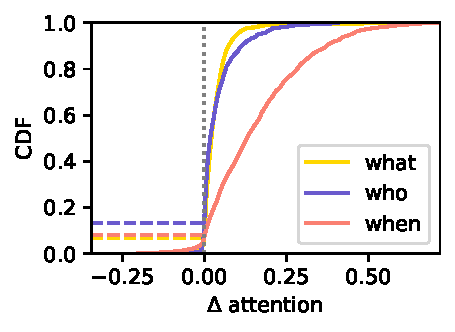
\includegraphics[width=0.95\textwidth]{Figures/attn_illustration_mistral.pdf} 
\end{minipage}
\caption{Depending on the question, the attention-eliciting prompt introduced in \cref{fig:prompt_short} induces attention focusing on different parts of the same response (``when'', ``who'' and ``what'').
In the plot on the right, we show the CDF of $\Delta_{attn}$, the change of attention weight on the corresponding concept when asked the relevant question, on all 1,024 heads of Mistral-7B.
For example, for ``when'', we compute $\Delta_{attn}$ as the attention weight on ``On July 20, 1969'' when asked the ``when'' question minus the average of the cases where the other two questions were asked.
%We then plot the CDF of such $\Delta_{attn}$ on all 1,024 heads of Mistral-7B.
In all cases, the attention significantly increases on the relevant tokens (p-value from one-sided t-test is at most 9e-90).
}
\label{fig:attnillustration}
\end{figure*}
}
\FigAttentionCase


\cref{fig:attnillustration} illustrates how the attention-eliciting prompt (\cref{fig:prompt_short}) induces varying emphases on the same response for different questions.
For instance, when the question focuses on ``when'', the section of the response detailing the event date receives greater attention weight across all heads. 
This indicates that the weighting scheme introduced in \cref{eq:main} effectively overweights relevant tokens and underweights irrelevant ones, resulting in a more contextualized version of sequence likelihood. %, which is a more suitable confidence measure.

Besides using a prompt, a more straightforward source of attention weights is the original generating process.
Specifically, when the LM completes generating $\predSeq$, we retrieve the attention for the next token.
We refer to this variant as \methodnameNext, in contrast to \methodnamePrompt with the prompt. 
Our hypothesis is that the LM induces some internal attention on the critical words of the generation even without an explicit prompt asking for it, and we will explain how to identify such attention in \cref{sec:method:headchoice}.


%TODO: use the same prompt for self-eval



\subsection{The Choice of Heads}\label{sec:method:headchoice}

%\cref{fig:attnillustration} illustrates that w
While the prompt can enhance overall attention on relevant tokens, averaging attention across heads---even with the prompt---is unwise. 
Many attention heads likely focus, for example, on ensuring grammatical correctness, with only a fraction dedicated to the response. 
Selecting only the useful heads from the multitude of heads (e.g., out of 1,600 in LLaMA2-13B) remains a challenging task.


%While it is possible to heuristically or manually pick a few heads in the LM for their attentions, a systematic approach is more desirable.
We present a systematic approach to identify the appropriate heads.
Let $w^h$  denote the attention weights from head $h$, and $\ConfMethod^h$ the associated confidence score computed via  \cref{eq:main}.
For each head $h$ and a subset of the samples, we use the associated confidence $\ConfMethod^h$ to predict the accuracy of responses, and compute an AUROC (similar to \citealp{kuhn2023semantic}), denoted as $\text{AUROC}_h$. 
Notably, we found that the ``functionality'' of the heads appears relatively stable: That is, if we compare the $\text{AUROC}_h$ on two subsets of the population, the ranking of these heads is highly consistent across the two subsets, as shown in \cref{fig:headvaltest}. 
As a result, we propose to pick the top $k=10$ heads on the validation dataset and average the attention weights of only these heads.
The reason why we pick more than one head is because picking only the best head is likely affected by noise due to the size of the validation set.
In \cref{sec:exp}, we show that leveraging the attention from about $k=10$ top heads performs better than either the average attention of all heads, or the top head.



\def \FigHeadConsistency{
\begin{figure}[ht]
\centering
% Text above the image
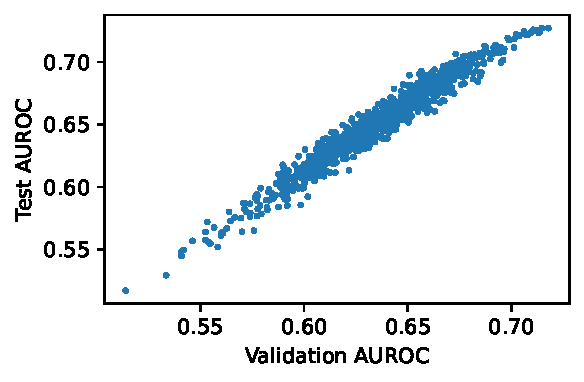
\includegraphics[width=0.42\textwidth]{Figures/head_consistency_mistral_nq_open_new.pdf} % Adjust 'width' as needed
% \vspace{-3mm}
\caption{
Scatter plot of test vs validation AUROC for confidence measures computed via \cref{eq:main} with different heads' attention weights, on Natural Questions (\datasetnqopen) %~\citep{kwiatkowski-etal-2019-natural} dataset 
with Mistral-7B model. %~\citep{jiang2023mistral} model.
% accurcy measured by LLaMA2-70B
The ranking is highly consistent---the best heads on the validation set continue to perform well on the test set. 
In this case, the Spearman correlation~\citep{spearman1961proof} is $>97\%$.
We can thus pick only a small subset of the 1024 heads (or more for other LMs) to construct the final confidence measure $\ConfMethod$.
}
\label{fig:headvaltest}
% \vspace{-4mm}
\end{figure}
}
\FigHeadConsistency
